\section{Kleenes sætning}
\subsection{Kleenes sætning del 1}
\begin{frame}
\frametitle{Status}
\begin{itemize}[<+->]
\item Vi har defineret 4 formalismer
regulære udtryk
FA,
NFA,
NFA-$\Lambda$
\item og er ved konstruktivt at bevise ækvivalens i udtrykskraft
\end{itemize}
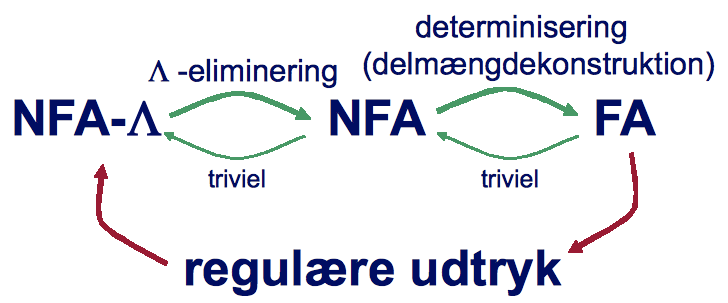
\includegraphics[scale=0.4]{images/2_seminar_equiv}
\end{frame}

\begin{frame}
\frametitle{Ethvert regulært udtryk kan oversættes til en NFA-$\Lambda$}
(Kleenes sætning, del 1)
\begin{itemize}
\item Bevis:
  Induktion i strukturen af det regulære udtryk $r$.
\item
Vis konstruktivt for hvert tilfælde hvordan man kan lave den korrekte NFA-$\Lambda$
\end{itemize}
\end{frame}
\begin{frame}
\frametitle{Basis}
\begin{columns}
\column{5cm}
\begin{itemize}
\item 
$r=\emptyset$
\item $r=\Lambda$
\item $r=a,$ hvor $a\in\Sigma$
\end{itemize}
\column{5cm}
\begin{itemize}[<+->]
\item
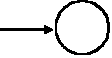
\includegraphics[scale=0.4]{images/2_seminar_basis_emptyset}
\item
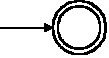
\includegraphics[scale=0.4]{images/2_seminar_basis_lambda}
\item
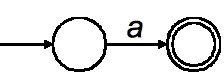
\includegraphics[scale=0.4]{images/2_seminar_basis_a}
\end{itemize}
\end{columns}
\end{frame}
\begin{frame}
\frametitle{Induktionsskridt}
\begin{itemize}[<+->]
\item For alle deludtryk $s$ af $r$ kan vi udnytte induktionshypotesen.
\item der eksisterer en NFA-$\Lambda$ $M_s$ hvor $L(M_s)=L(s)$
\item 
\begin{columns}
\column{5cm}$r=r_1+r_2$ \pause
\column{5cm}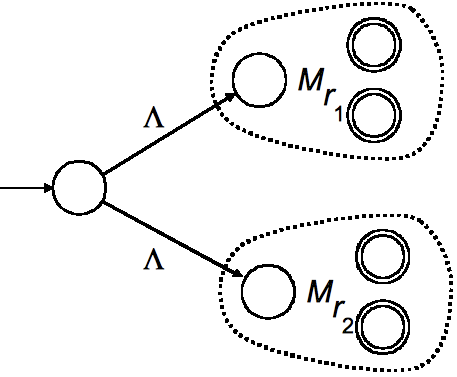
\includegraphics[scale=0.4]{images/2_seminar_kleene_1_add}
\end{columns}
\end{itemize}
\end{frame}
\begin{frame}
\frametitle{Induktionsskridt (part 2)}
\begin{columns}
\column{5cm}$r=r_1\cdot r_2$ \pause
\column{5cm}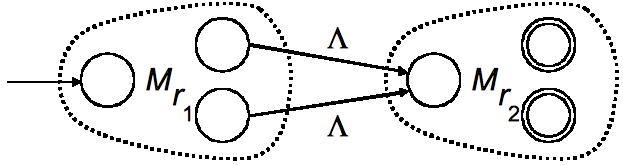
\includegraphics[scale=0.4]{images/2_seminar_kleene_1_times}
\end{columns} \pause
\begin{columns}
\column{5cm}$r=r_1^*$ \pause
\column{5cm}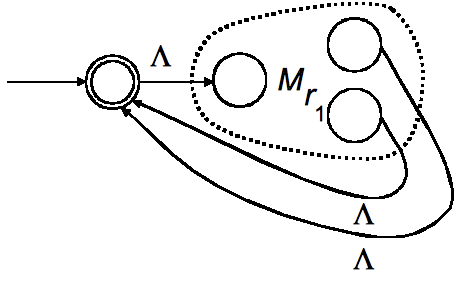
\includegraphics[scale=0.4]{images/2_seminar_kleene_1_star}
\end{columns}
\end{frame}

\begin{frame}
\frametitle{Formel beskrivelse og bevis for korrekthed}
Se beviset i bogen: p. 146
\end{frame}

\begin{frame}
\frametitle{Eksempel}
Konstruer en NFA-$\Lambda$ for det regulære udtryk $(00+1)^*(10)^*$
\begin{itemize}[<+->]
\item 0:
  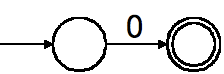
\includegraphics[scale=0.4]{images/2_seminar_kleene_1_ex_0}
\item 1:
  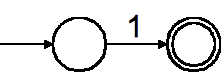
\includegraphics[scale=0.4]{images/2_seminar_kleene_1_ex_1}
\item 00:
  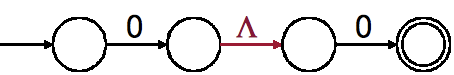
\includegraphics[scale=0.4]{images/2_seminar_kleene_1_ex_00}
\item 10:
  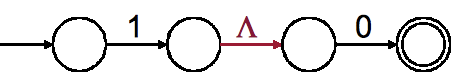
\includegraphics[scale=0.4]{images/2_seminar_kleene_1_ex_10}
\end{itemize}
\end{frame}
\begin{frame}
\frametitle{Eksempel fortsat}
Konstruer en NFA-$\Lambda$ for det regulære udtryk $(00+1)^*(10)^*$
\begin{itemize}[<+->]
\item $00+1$:
  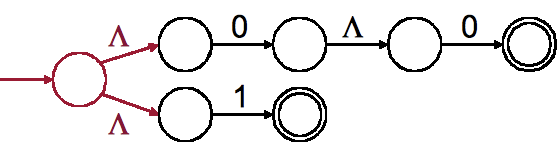
\includegraphics[scale=0.4]{images/2_seminar_kleene_1_ex_00plus1}
\item $(00+1)^*$:
  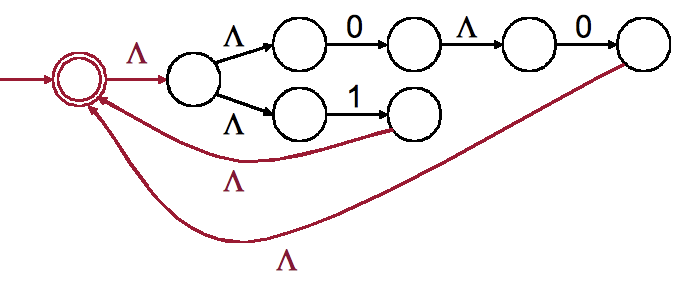
\includegraphics[scale=0.4]{images/2_seminar_kleene_1_ex_00plus1star}
\end{itemize}
\end{frame}
\begin{frame}
\frametitle{Eksempel fortsat}
Konstruer en NFA-$\Lambda$ for det regulære udtryk $(00+1)^*(10)^*$
\begin{itemize}[<+->]
\item $(10)^*$:
  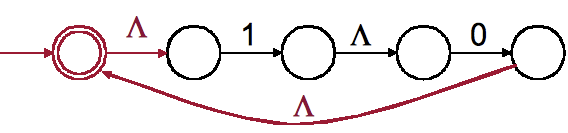
\includegraphics[scale=0.4]{images/2_seminar_kleene_1_ex_10star}
\item $(00+1)^*(10)^*$:
  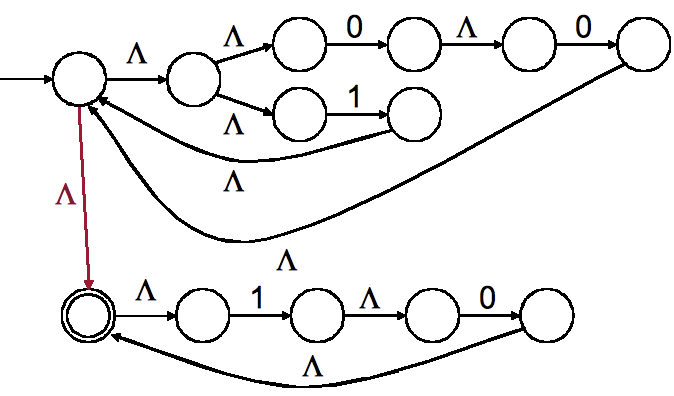
\includegraphics[scale=0.4]{images/2_seminar_kleene_1_ex_00plus1star10star}
\end{itemize}
\end{frame}
\begin{frame}
\frametitle{Øvelser}
\begin{itemize}
\item [Martin] Opg. 4.35 (a) (p. 163)\\
Udfør algoritmen for konstruktion af NFA-$\Lambda$ fra regulært udtryk. 
\end{itemize}
\end{frame}
\subsection{Kleenes sætning del 2}
\begin{frame}
  \frametitle{Enhver FA kan oversættes til et regulært udtryk}
Kleene's sætning del 2.

Vi laver bevis med induktion naturligvis, men induktion i hvad?
\end{frame}

\begin{frame}
\frametitle{Fra FA til regulært udtryk}
\begin{itemize}[<+->]
\item For en FA $M=(Q, \Sigma , q_0, A, \delta )$ er $L(M)$ defineret som
	$L(M) = \{ x\in \Sigma^* | \delta^*(q_0, x)\in A \}$
\item Da A er endelig kan L(M) udtrykkes som en endelig forening af sprog på form
	 $L(p, q) = \{ x\in \Sigma^* | \delta^*(p, x)=q \}$
\item Vi vil vise at hvert af disse sprog kan oversættes til et regulært udtryk, $r(p, q)$, og derefter kombinere disse med “+”
\end{itemize}
\end{frame}
\begin{frame}
\frametitle{Induktion i antal tilstande}
\begin{itemize}[<+->]
\item Antag tilstandene i M er nummereret $1, ..., |Q|$
\item Definer $L(p, q, k)$ hvor $p,q\in Q$ og $k\in \{1..|Q|\}$ som
  mængden af strenge, der fører fra p til q og kun går gennem
  tilstande med nummer $\leq k$ (fraregnet endepunkterne)
  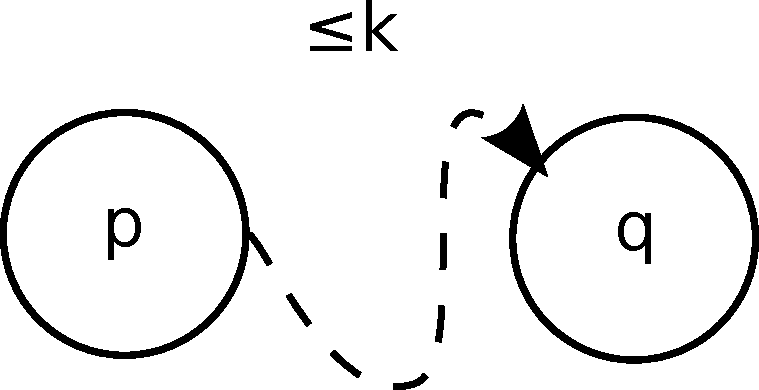
\includegraphics[scale=0.2]{images/2_seminar_kleene_2_lessk}
\item dvs.  $L(p, q) = L(p, q, |Q|)$
\item Vi vil vise ved induktion i $k$ at $L(p, q, k)$ svarer til 
et regulært udtryk, $r(p, q, k)$
\item dvs. vælg  $r(p, q) = r(p, q, |Q|)$
\end{itemize}
\end{frame}
\begin{frame}
\frametitle{Basis}
$k = 0$
\begin{itemize}[<+->]
\item 
$L(p, q, 0)$ er mængden af strenge, der fører fra 
$p$ til $q$ uden at gå gennem nogen tilstande 
(fraregnet endepunkterne)
\item
hvis $p\neq q$: 
$L(p, q, 0) = \{ a\in \Sigma  | \delta (p, a) = q \}$
\item
hvis $p=q$: 
$L(p, q, 0) = \{ a\in \Sigma  | \delta (p, a) = p \} \cup \{\Lambda\}$
\item
dvs. vi kan altid finde et regulært udtryk 
$r(p, q, 0)$ for $L(p, q, 0)$
\end{itemize}
\end{frame}
\begin{frame}
\frametitle{Induktionsskridt}
$k+1$
\begin{itemize}[<+->]
\item $L(p, q, k + 1)$ er mængden af strenge, der fører fra $p$ til $q$ 
og kun går gennem tilstande med nummer $\leq k + 1$
\item
To tilfælde:

\begin{itemize}[<+->]
\item 
  Strenge der ikke går gennem tilstand $k + 1$: $L(p, q, k)$ 
\item Strenge
  der går gennem tilstand $k + 1$: $L(p, k + 1, k) L(k + 1, k + 1, k)^*
  L(k + 1, q, k)$
\end{itemize}
\item dvs. $L(p, q, k + 1) = L(p, q, k) \cup 
			    L(p, k + 1, k) L(k + 1, k + 1, k)^* L(k + 1, q, k)$
\item som vha. induktionshypotesen svarer til et regulært udtryk 
	$r(p, q, k + 1) = r(p, q, k) + 
			    r(p, k + 1, k) r(k + 1, k + 1, k)^* r(k + 1, q, k)$
\end{itemize}
\end{frame}
\begin{frame}
\frametitle{Eksempel}
Oversæt denne FA til et regulært udtryk
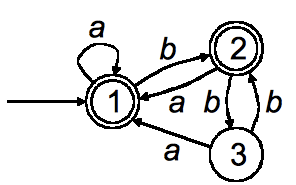
\includegraphics[scale=0.4]{images/2_seminar_kleene_2_ex.png}
\begin{itemize}[<+->]
\item $r = r(1,1,3) + r(1,2,3)$
\item $r(1,1,3) = r(1,1,2) + r(1,3,2)r(3,3,2)^*r(3,1,2)$
\item $r(1,1,2) = r(1,1,1) + r(1,2,1)r(2,2,1)^*r(2,1,1)$
\item $r(1,1,1) = r(1,1,0) + r(1,1,0)r(1,1,0)^*r(1,1,0)$
\item $r(1,1,0) = a + \Lambda$
\item Heldigvis kan vi sætte en computer til det!
\end{itemize}
\end{frame}
\begin{frame}
\frametitle{Eksempel fortsat}
\begin{itemize}[<+->]
\item \tiny{$r = ((\emptyset+(((((\emptyset +a)+\lambda)+(\emptyset (((\emptyset +\lambda )^*)$$(\emptyset +a))))+((((\emptyset +a)+\lambda )+(\emptyset (((\emptyset +\lambda )^*)(\emptyset +a) )))$$(((((\emptyset +a)+\lambda )+(\emptyset (((\emptyset +\lambda )^*)(\emptyset +a))))^*)(((\emptyset +a)+\lambda )+(\emptyset (((\emptyset +\lambda )^*)(\emptyset +a)))))))+((((\emptyset +b)+(\emptyset (((\emptyset +\lambda )^*)(\emptyset +b))))+((((\emptyset +a)+\lambda )+(\emptyset (((\emptyset +\lambda )^*)(\emptyset +a))))(((((\emptyset +a)+\lambda )+(\emptyset (((\emptyset +\lambda )^*)(\emptyset +a))))^*)((\emptyset +b)+(\emptyset (((\emptyset +\lambda )^*)(\emptyset +b)))))))(((((\emptyset +\lambda )+((\emptyset +b)(((\emptyset +\lambda )^*)(\emptyset +b))))+(((\emptyset +a)+((\emptyset +b)(((\emptyset +\lambda )^*)(\emptyset +a))))(((((\emptyset +a)+\lambda )+(\emptyset (((\emptyset +\lambda )^*)(\emptyset +a))))^*)((\emptyset +b)+(\emptyset (((\emptyset +\lambda )^*)(\emptyset +b)))))))^*)(((\emptyset +a)+((\emptyset +b)(((\emptyset +\lambda )^*)(\emptyset +a))))+(((\emptyset +a)+((\emptyset +b)(((\emptyset +\lambda )^*)(\emptyset +a))))(((((\emptyset +a)+\lambda )+(\emptyset (((\emptyset +\lambda )^*)(\emptyset +a))))^*)(((\emptyset +a)+\lambda )+(\emptyset (((\emptyset +\lambda )^*)(\emptyset +a)))))))))))+((((\emptyset +b)+(\emptyset (((\emptyset +\lambda )^*)(\emptyset +b))))+((((\emptyset +a)+\lambda )+(\emptyset (((\emptyset +\lambda )^*)(\emptyset +a))))(((((\emptyset +a)+\lambda )+(\emptyset (((\emptyset +\lambda )^*)(\emptyset +a))))^*)((\emptyset +b)+(\emptyset (((\emptyset +\lambda )^*)(\emptyset +b)))))))+((((\emptyset +b)+(\emptyset (((\emptyset +\lambda )^*)(\emptyset +b))))+((((\emptyset +a)+\lambda )+(\emptyset (((\emptyset +\lambda )^*)(\emptyset +a))))(((((\emptyset +a)+\lambda )+(\emptyset (((\emptyset +\lambda )^*)(\emptyset +a))))^*)((\emptyset +b)+(\emptyset (((\emptyset +\lambda )^*)(\emptyset +b)))))))(((((\emptyset +\lambda )+((\emptyset +b)(((\emptyset +\lambda )^*)(\emptyset +b))))+(((\emptyset +a)+((\emptyset +b)(((\emptyset +\lambda )^*)(\emptyset +a))))(((((\emptyset +a)+\lambda )+(\emptyset (((\emptyset +\lambda )^*)(\emptyset +a))))^*)((\emptyset +b)+(\emptyset (((\emptyset +\lambda )^*)(\emptyset +b)))))))^*)(((\emptyset +\lambda )+((\emptyset +b)(((\emptyset +\lambda )^*)(\emptyset +b))))+(((\emptyset +a)+((\emptyset +b)(((\emptyset +\lambda )^*)(\emptyset +a))))(((((\emptyset +a)+\lambda )+(\emptyset (((\emptyset +\lambda )^*)(\emptyset +a))))^*)((\emptyset +b)+(\emptyset (((\emptyset +\lambda )^*)(\emptyset +b))))))))))) $}
\item (Hvis programmet ikke simplificerer undervejs...)
\end{itemize}
\end{frame}
\begin{frame}
\frametitle{Øvelser}
\begin{itemize}
\item [Martin] Opg. 4.38(b) (p. 164)\\
Brug algoritmen fra Kleenes sætning del 2.
\end{itemize}
\end{frame}
